%!TEX root =  main.tex

\section{Background}

In this section we give a short introduction to the Governed Components (GC) language~\cite{Hugo} that is used in this paper as the reference model for reactive components. The language used here is a fragment of the one introduced in~\cite{Hugo} (excluding the specification of alternative behaviours in protocols), serving as a proof-of-concept of our approach and already presenting challenging features. In the remainder of the section we present the syntax and semantics of the language.



\subsection{Syntax of Governed Components} \label{Syntax of Governed Components}


The language syntax is shown in Table~\ref{syntaxcomponents}. There are two kinds of components ($K$) in the language: base and composite. Both kinds interact with the external environment by means of ports exposed as the component interface. Port identifiers are ranged over by $x,y,z,u,w$ and we write $[\tilde{x}>\tilde{y}]$ to represent an interface comprising input ports ($\tilde{x}$ which abbreviates $x_1, \ldots, x_k$) and output ports ($\tilde{y}$). Components receive values on the input ports and emit values on the output ones. Besides of the interface, components are defined by their implementation. 

In the case of a base component the implementation is given by local binders ($L$). A local binder specifies a function, denoted as $y=f(\tilde{x})$, which is used to compute (output) values for the port $y$  (abstracting from how $f$ is defined) relying on values received on (input) ports $\tilde{x}$. Lists of local binders are captured by the composition $L,L$, so an implementation of a base component may have one or more local binders (notice that the empty list of binders is excluded in the syntax but is immediate to add).


\begin{table}[t]
    \centering
    \begin{tabular}{l l l l l}
    Components & $K$  & ::=& 
    $\chorboxb {\tilde x}{\tilde y}{L}$
    %[\tilde{x}>\tilde{y}]\{L\}$ 
    & base\\
         &     &    & $\chorbox{\tilde x}{\tilde y}{D}{\role r[F]}{R}{G}$ & composite\\
    
    
    
    Local Binders & $L$ & ::=& $y=f(\tilde{x})$ & \\
    & & $\ \ \ |$ & $L,L$ & \\
    
    Protocol  & $G$ & ::=& $\gcom p \lab{\tilde  q};G$ & communication\\
    & & $\ \ \ |$ & $\mu \recvar{X}.G$ & recursion\\
    & & $\ \ \ |$ & $\recvar{X}$ & recursion variable \\
    & & $\ \ \ |$ & $\gend$ & termination\\
    
    
    Role assignments &  $R$ &::= & $\role p=K$ & \\
    & & $\ \ \ |$ & $R,R$ & \\
    
    
   Connection Binders  & $D$ & ::=& $\dbinder{\lab}{p}{x} {\roleport{q}{y}}$ & \\
    & & $\ \ \ |$ & $D,D$ & \\
    
   
   
   Forwarders  & $F$ &::= & $z\leftarrow w $ & \\
   & & $\ \ \ |$ & $F,F$ &\\
   & & & & \\
   
    \end{tabular}\\
    
    \caption{Syntax of Governed Components}
    
    \label{syntaxcomponents}
    
\end{table}


The implementation of a composite component, represented by $\{G;R;D;r[F]\}$, is an assembly of subcomponents which interaction is governed by a predefined protocol ($G$). Besides of the protocol, 
composite components specify the set of subcomponents, which are given in $R$ together with their \emph{roles} in the interaction, and a list of (distribution) binders ($D$) that provide an association between
the messages exchanged in the protocol and the ports in components. Finally, the subterm $r[F]$ is used to describe externally-observable behaviour: the (only) subcomponent responsible for the interaction with the composite component's external environment is identified (by its role $\role r$) and the respective connection between ports is provided ($F$). We often refer to such a subcomponent as the interfacing one. The idea is that values received on the (input) ports of the composite component are directly forwarded to the (input) ports of the interfacing subcomponent, and values emitted on the (output) ports of the interfacing subcomponent are forwarded to the (output) ports of the composite component. 

We now describe each of the remaining syntactic categories of Table~\ref{syntaxcomponents} that are used in the implementation of composite components.
Forwarders ($F$) are of the form $z\leftarrow w$ and specify that values flow from port $w$ to port $z$, which may be used for both input and output forwarding (e.g., Figure~\ref{forwarders} depicts the forwarders $x'\leftarrow x$ and $y\leftarrow y'$). Lists of forwarders are captured by the composition $F,F$, where we exclude the possibility of having an empty list (components defined with an empty list of forwarders cannot interact with the environment, which can nevertheless be modelled here).

\begin{figure}[t]

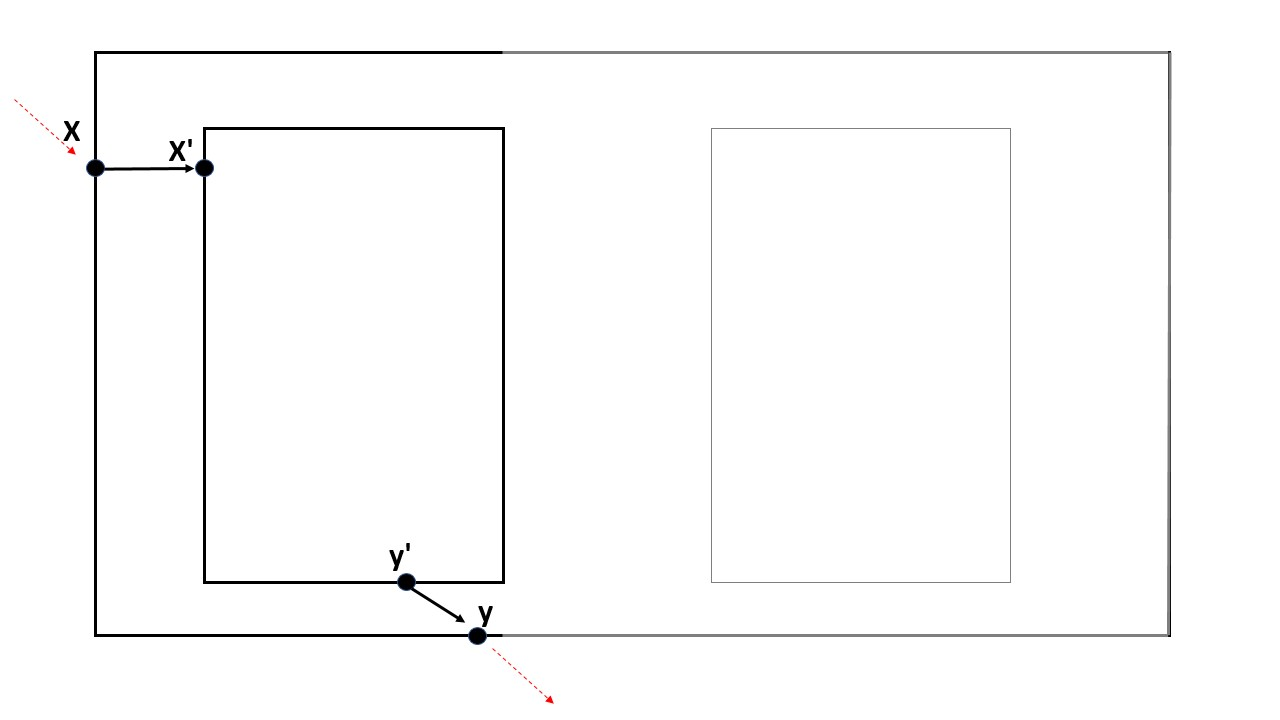
\includegraphics[width=6cm]{forwarders.jpg}
\centering
\caption{Graphic illustration of forwarders.
\label{forwarders}}


\end{figure}

Protocol specifications ($G$) prescribe the interaction among a set of roles, ranged over by $\role p,\role q,\role r$. The communication term $\gcom p \lab{\tilde  q};G $ specifies that role $\role p$ sends the message labelled  $\lab$  to the nonempty set of roles $\tilde{\role q}$, after which the protocol continues as specified by $G$. Terms $\mu X.G$ and $X$ specify infinite behaviour via the standard combination of the recursive protocol construct and recursion variables. The $\gend$ term defines the inactive protocol. As previously mentioned, the difference with respect to~\cite{Hugo} (and other global protocol languages) is the absence of branching.

Each subcomponent of the composite component is associated to a role used in the protocol as specified in role assignments ($R$). The term $\role p=K$ declares that component $K$ is the implementation of the role $\role p$. We can have one (more likely two, since we are composing components) or more role assignments in a list ($R,R$). The idea is that subcomponents interact among them as prescribed in the protocol, taking into account the correspondence given by the role identifiers. 

 Connection binders $D$ specify the correspondence between ports of a component and messages also relying on the role identifiers. 
  The connection binder $\dbinder{\lab}{p}{y} {\roleport{r}{x}}$ declares that the message labelled as $\lab$ carries values sent from port $y$ of role $\role p$ that are to be received on port $x$ of role $\role r$. 
  The idea is that ports are uniquely associated to message labels $\lab$, so that each communication step in the protocol (either output or an input) has a precise mapping to a port.

%SYNTACTIC CONSTRAINTS / CONVENTIONS
% - DISTRIBUTION BINDERS determine unique association between outport and message label, and inports are uniquely associated to message labels
% - output ports in base components have a corresponding local binder definition
% - ...

%%%%%%%%%%%%%%%%%%%%%%%%%%%%  
% SEMANTICS - BASE COMPONENTS
%%%%%%%%%%%%%%%%%%%%%%%%%%%%  

\subsection{Semantics of Governed components}

We now present the operational semantics of the GC in a terms of a labelled transition system (LTS).  We denote by $K \lto{\lambda} K'$ that component $K$ evolves in one computational step to $K'$, where observations are captured by labels defined as follows $\lambda::=x?v\ |\ y!v\ |\ \tau$. Transition label $x?v$ represents an input on port $x$ of a value $v$, label $y!v$ captures an output on port $y$ of value $v$, and label $\tau$ denotes an internal move. The rules that describe the behaviour of components are presented in two parts, addressing base and composite components separately.

\begin{itemize}
    \item Semantics of base components


The rules defining the semantics of base components are displayed in Table~\ref{tab:gc_semantics_base}. 
%
The two main rules $\m{OutBase}$ and $\m{InpBase}$ address base components, and are defined relying on transitions exhibited by local binders, denoted $L \lto{\lambda} L'$, that are also shown in Table~\ref{tab:gc_semantics_base}. 

Rule $\m{OutBase}$ states that if the
local binders $L$  can output a value $v$ on port $y$, which is part of the component's interface,
then the corresponding output is exhibited by the base component.
%
Notice that the transition of the local binder specifies a final configuration $L'$ which is accounted for in the evolution of the base component.
%
Rule $\m{InpBase}$ follows the same lines to model an input.


The remaining rules describe the behaviour of local binders, where values to be sent are computed based on received ones. A local binder $y=f(\tilde{x})$ may produce an output value to be sent on port $y$, when all the values required by $f$ have been received, (at least) one for each $x$ in $\tilde{x}$. 
%
Furthermore, taking into account that received values are to be processed in a first-in first-out (FIFO) discipline, we need to introduce queues in runtime local binders.
In order to keep values received on different ports in a corresponding order of arrival, each element in a queue is a store defined as a partial mapping from ports to values.
%
We write $\tilde \sigma$ to abbreviate a queue of stores $\sigma_1, \sigma_2, \ldots, \sigma_k$,
where in $\sigma_1$ the oldest values received are stored, in $\sigma_2$ the second-oldest values, and so on and so forth up to $\sigma_k$. 
%
The syntax of runtime local binders includes queues of stores as follows $L::=\lbinder{y}{\tilde{\sigma}}{f(\tilde{x})}\ |\ L,L$.
%
We remark that the values stored in the queues are the only ones needed to compute the respective functions, so in local binder $\lbinder{y}{\tilde{\sigma}}{f(\tilde{x})}$ we have that each $\sigma_i$ only stores values for ports $\tilde{x}$.










\begin{table}[t]
\centering
\begin{tabular} {c c c}

        \infer[\m{OutBase}]
        {
        \chorboxb {\tilde x}{\tilde y}{L}
        \lto{y!{v}{}}
        \chorboxb {\tilde x}{\tilde y}{L'}
        }
        {
        L
        \lto{y!{v}{}{}}
        L'
        & y \in \tilde y
        }
 & &

        \infer[\m{InpBase}]
        {
        \chorboxb {\tilde x}{\tilde y}{L}
        \lto{x?v}
        \chorboxb {\tilde x}{\tilde y}{L'}
        }
        { L \lto{x?v} L' & x \in \tilde x }
\\

& & \\
           \infer[\m{LConst}]
            {
            \lbinder y{\cdot} {\mathit{f}()}
            \lto{{y}!{v}}
            \lbinder y{\cdot}{\mathit{f}()}}
        {f() \eval v}
& &
            \infer[\m{LOut}]
            {
            \lbinder y{\sigma,{\tilde\sigma}} {\mathit{f}(\tilde{x})}
            \lto{{y}!{v}}
            \lbinder y{\tilde \sigma}{\mathit{f}(\tilde{x})}
            }
        {
			\{\tilde x\} {=} \dom(\sigma) & f(\sigma(\tilde x)) \eval v
        }
\\ 

& & \\


\multicolumn{3}{c}{
\infer[\m{LInpNew}]
{
\lbinder y{\tilde\sigma}{f(\tilde{x})}
\lto{{x}?{v}}
\lbinder y{\tilde\sigma,\{x \mapsto v\}} {f(\tilde{x})}
}
{
x \in \bigcap_{\sigma_i \in \tilde \sigma}\dom(\sigma_i)
&
x \in \tilde x
} }
\\

& & \\

 \multicolumn{3}{c}{	\infer[\m{LInpUpd}]
        {
        \lbinder y{\tilde\sigma_1,\sigma,\tilde\sigma_2} {f(\tilde{x})}
       \lto{{x}?{v}}
        \lbinder y{\tilde\sigma_1,\sigma[x \mapsto v],\tilde\sigma_2} {f(\tilde{x})}
        }
        {
		x \in \bigcap_{\sigma_i \in \tilde \sigma_1}\dom(\sigma_i)
		&
		x \not\in \dom(\sigma)
		&
		x \in \tilde x
        } }
\\

& & \\

  \multicolumn{3}{c}{ \infer[\m{LInpDisc}]
{
	\lbinder y{\tilde\sigma} {f(\tilde{x})}
       \lto{{x}?{v}}
    \lbinder y{\tilde\sigma} {f(\tilde{x})}
}
{
	x \not\in \tilde x
} }
\\

& & \\

\infer[\m{LOutLift}]
       {
       L_1, L_2
       \lto{{y}!{v}}
       L_1', L_2
       }
       {
	L_1 \lto{{y}!{v}}L_1'}
 & &
       \infer[\m{LInpList}]
       {
       L_1, L_2
       \lto{{x}?v}
       L_1', L_2'
       }
       {
	L_1 \lto{{x}?v}L_1'
	&
	L_2 \lto{{x}?v}L_2'}\\
	
	& & \\
\end{tabular}
  \caption{Semantics of base components}
  \label{tab:gc_semantics_base}
\end{table}

%%%%%%%%%%%%%%%%%%%%%%%%%%%%  
% SEMANTICS - COMPOSITE COMPONENTS
%%%%%%%%%%%%%%%%%%%%%%%%%%%%  

Rule $\m{LConst}$ captures the behaviour of binders that require no inputs, i.e., when the respective functions have no parameters. This means that the local binder can
always output the (constant) value computed by the function. In the rule we denote by $\cdot$ the empty queue (since no values are required none are stored)
and by $f() \eval v$ that function $f$ evaluates to value $v$ (from which computation we abstract from).

Rule $\m{LOut}$ states that if all parameters (considering a nonempty set) of the function specified in the binder have a mapping in the oldest store of
the queue, then the local binder can output the value computed by the function. As a result of the output, the oldest store is removed from the queue.
We use $ \dom(\sigma)$ to refer to the domain of mapping $\sigma$, and $\sigma(\tilde x)$ to represent the values mapped by $\sigma$ of ports $\tilde x$ 
(e.g., $\sigma(x_1, x_2) = v_1, v_2$ when $\sigma = \{x_1 \mapsto v_1, x_2 \mapsto v_2\}$) which are used to evaluate the function.

The following rules describe how queues are manipulated so as to address input transitions of local binders. 
Rule $\m{LInpNew}$ captures the case when a new store has to be added, namely when every store in the queue already has a mapping 
for that port ($x \in \bigcap_{\sigma_i \in \tilde \sigma}\dom(\sigma_i)$)  or when the queue is empty ($\tilde \sigma = \cdot$).
Notice that the resulting queue $\tilde{\sigma},\{x \mapsto v\}$ is the result of adding to the original queue $\sigma$ the new (singleton) store $\{x \mapsto v\}$.
%
Rule $\m{LInpUpd}$ describes the case when the value received is used to update a store, namely the oldest store in the queue  that does not have a mapping for that port.
%
Notice that for both $\m{LInpNew}$ and $\m{LInpUdp}$ it must be the case that the port where the value is received is actually a parameter of the function, and
otherwise received values are discarded, as specified in rule $\m{LInpDisc}$.

Rule $\m{LOutLift}$ states that if a binder can output a value on a port so can the list of binders, which means that local binders can output in an interleaved way.
Instead, rule $\m{LInpList}$ says that all binders react to an input on a port in a synchronised way, so as to ensure that every local binder that uses that port receives a copy of the value.

\item{Semantics of composite components}


%After presenting the rules that describe the behaviour of base components, 
We now introduce the rules that capture the behaviour of composite components, displayed in Table~\ref{tab:gc_semantics_composite}. 
%
Note that a composite component may itself be used as a subcomponent of another composition (of a ``bigger'' component), while base components are the syntactic leaves.
%Note: We start from  base components and putting them together with the protocol  we obtain a composite component, that can be further used as a subcomponent of some other (``bigger'') 
%composite component, and so, and so one. 
%
The first three rules of Table~\ref{tab:gc_semantics_composite} capture the internal behaviour of composite components, while the remaining two describe the externally-observable behaviour.








\begin{table}[t]
\centering
\begin{tabular}{c}

    
        \infer[\m{OutChor}]
        {\chorbox{\tilde x}{\tilde y}{ D}{\role{r}[ F]}{\roleas{p}{K}, R}{G}
	\lto{\tau}
        \chorbox{\tilde x}{\tilde y}{ D}{\role{r}[ F]}{ \roleas{p}{K'}, R}{G'}}        
	{K \lto{{u}!{v}{}} K' \qquad 
	D = \dbinder{\lab}{q}{z} {\roleport{p}{u}}, D'
        \qquad
        G \lto{\labout{\role p}{\lab}{v}} G'
        }
\\

\\


        \infer[\m{InpChor}]
        {\chorbox{\tilde x}{\tilde y}{ D}{\role{r}[ F]}{ \roleas{q}{K},  R}{G}
	\lto{\tau}
        \chorbox{\tilde x}{\tilde y}{ D}{\role{r}[ F]}{\roleas{q}{K'},  R}{G'}}        
	{
        K \lto{{z}?v} K' \qquad
         D = \dbinder{\lab}{q}{z} {\roleport{p}{u}},  D' \qquad
        G \lto{\labinp{\role q}{\lab}{v}} G'
	}
\\

\\


	\infer[\m{Internal}]
	{\chorbox{\tilde x}{\tilde y}{ D}{\role{r}[ F]}{\roleas{s}{K},  R}{ G}
	\lto{\tau}
	\chorbox{\tilde x}{\tilde y}{ D}{\role{r}[ F]}{ \roleas{s}{K'},  R}{G}}	
	{K \lto{\tau} K'}
\\

\\


	\infer[\m{OutComp}]
	{
	\chorbox {\tilde x}{\tilde y}{ D}{\role{r}[ F]}{\roleas{r}{K},  R}{G}
	\lto{{y}!{v}{}}
	\chorbox {\tilde x}{\tilde y}{ D}{\role{r}[ F]}{\roleas{r}{K'},  R}{G}
	}	
	{
	K\lto{{z}!{v}{}{}} K'
	\qquad
	F = \fbinder {y}z ,  F'
	\qquad
	y \in \tilde y
	}
\\

\\


        \infer[\m{InpComp}]
        {\chorbox{\tilde x}{\tilde y}{ D}{\role{r}[ F]}{\roleas{r}{K}, R}{G}
	\lto{{x}?v}
        \chorbox{\tilde x}{\tilde y}{ D}{\role{r}[ F]}{ \roleas{r}{K'}, R}{G}}        
	{ 
	K \lto{{z}?v} K'  \qquad  F = \fbinder z{x},  F' \qquad x \in \tilde x
	}\\
	
	\\
	
	
\end{tabular}
  \caption{Semantics of composite components.}
  \label{tab:gc_semantics_composite}
\end{table}




Rules $\m{OutChor}$ and $\m{InpChor}$ capture the interaction among subcomponents of a composite component. 
Rule $\m{OutChor}$ addresses the case when a component is sending a message to another one. The premises, together with the role assignment $\roleas{p}{K}$, establish the connection among the sender component $K$, the component port $u$, the sender role $\role{p}$, and the message label $\lab$.
Premise $K \lto{{u}!{v}{}} K'$ says that the sender component ($K$) can perform an output of  value $v$ on port $u$. Premise $D = \dbinder{\lab}{q}{z} {\roleport{p}{u}}, D'$ says that the connection binders specify the relation between port $u$ of the sender role $\role{p}$ and message label $\lab$, and also with some receiver role ($\role{q}$) and associated port ($z$).
%
The last premise $G \lto{\labout{\role p}{\lab}{v}} G'$ realises the component governing by the protocol, i.e., saying that the communication is only possible if the protocol prescribes it. Namely, the premise says that the protocol exhibits an output of a value $v$ carried in message $\lab$ from role $\role{p}$. %($\labout{\role p}{\lab}{v}$). 
The rules for protocol transitions will be given afterwards. 
Notice that the transitions of component $K$ and the protocol $G$ specify final configurations $K'$ and $G'$  which are accounted for in the evolution of the composite component. 
 
 Rule $\m{InpChor}$ is similar, but instead of message sending, it addresses the case when a subcomponent receives a message from another subcomponent. The premises are equivalent to the ones for the rule $\m{OutChor}$, but now regard reception. Namely, by saying that the receiving component $K$ can exhibit the respective input transition, that the connection binder specifies the relation of message label $\lab$ with the receiver role $\role{q}$ and port $z$, and that the protocol $G$ prescribes the input of a value. 
 
 Rule $\m{Internal}$ allows for internal actions in a subcomponent ($K$), where the final configuration ($K'$) is registered in the final configuration of the composite component.
%
Rules $\m{OutComp}$ and $\m{InpComp}$ capture the interaction between a composite component and the external environment, realised by the interfacing subcomponent. The role assignment $\roleas{r}{K}$ captures the relation between component $K$ and the role $r$, which is specified as the interfacing role ($\role{r}[ F]$). Rule $\m{OutComp}$ allows for the interfacing component $K$ to send a value $v$ to the external environment via one of the ports of the composite component ($y$). Notice that the connection between the port of the interfacing component ($z$) and the port of the composite component ($y$) is specified in a forwarder ($F = \fbinder {y}z ,  F'$). Rule $\m{InpComp}$ follows the same lines to model an externally-observable input.

In rules $\m{InpChor}$ and $\m{OutChor}$ we specify protocol transitions which are described in the rules shown in Table~\ref{tab:g_semantics}. The respective labels are of the form $\labout{\role p}{\lab}{v}$ and $ \labinp{\role p}{\lab}{v}$. The former states that role $\role{p}$ sends value $v$ on message $\lab$ and the second one that role $\role{p}$
receives value $v$ on message $\lab$. We use $\alpha$ to range over protocol transitions, and use $\m{role}(\alpha)$ to refer to the role specified in label $\alpha$, i.e.,
 $\m{role}(\labout{\role p}{\lab}{v})=\m{role}(\labinp{\role p}{\lab}{v})=\role{p}$. 

In order to capture the behaviour of the components at runtime we need to store intermediate communication states, so we expand the syntax of protocols with runtime terms:

\begin{center}
    $G::=\dots \ | \ \gcom {} {\lab,v}{\tilde  q};\,G $
\end{center}

The term above denotes that the value $v$ has been sent on message $\lab$ by the sender, but still not received by (all of) the receivers ($\tilde{\role q}$). Hence, the (runtime) intermediate communication states originate in the emission of a message by the sender component and subsist up to the point all recipient components have received the message, registering in the meanwhile the communicated value in the protocol syntax.

We may now present the semantics of protocols given by the rules shown in Table~\ref{tab:g_semantics}. Rule $\m{GSVal}$ models an output of a message  $\lab$ from role $\role p$ that is sent to (possibly) multiple roles $\tilde{\role q}$. The transition label $\lto{\labout{\role p}{\lab}{v}}$ registers the sender role, the message label and the communicated value which is ``guessed'' at this point (as in the early semantics of the $\pi$-calculus~\cite{sangiorgowalker}). The final configuration is the (runtime) term $ \gcom {} {\lab,v}{\tilde  q}$ which registers both the message label $\lab$ together with the in-transit value ${v}$ and the list of recipients of the message $\tilde{\role q}$. 

Instead, rule $\m{GRVal}$ models an input: if there is a value in transit for a message (that has already been sent by some sender component) it can be received by one of the prescribed receivers ($\role q$), while the other receivers ($\tilde{\role q}$) remain waiting for the reception the message. That means that values that are sent on the same message are received by the recipients one by one. In the case of the reception when only one recipient is specified, then the
protocol proceeds with the intended continuation as described in rule $\m{GRVal2}$. Rule $\m{GRec}$ captures the recursion in a standard way, where the recursive protocol exhibits the transitions of its
unfolding. Rules $\m{GConc1}$ and $\m{GConc2}$ model concurrent and asynchronous execution of protocols, like  full $\beta$-reduction terms in $\lambda$-calculus. If the protocol can execute an action that does not involve a role in the prefix of the protocol, then the transition exhibited by the continuation is also exhibited by the prefixed protocol (without affecting the prefix). These two rules state that two interactions that involve separate roles do not interfere (an interpretation which is standard in choreographic models such as~\cite{fabrizio}).
 









\end{itemize}
%%%%%%%%%%%%%%%%%%%%%%%%%%%%  
% SEMANTICS - PROTOCOLS
%%%%%%%%%%%%%%%%%%%%%%%%%%%%  







\begin{table}[t]
\centering
\begin{tabular} {c c }

    \infer[\m{GSVal}]
    {
    \gcom p \lab{\tilde  q};\,G
    \ \lto{\labout{\role p}{\lab}{v}}\
    \gcom {} {\lab,v}{\tilde  q};\,G
    }
   {}
    
    & 
    
    
    
    
    \infer[\m{GRVal}]
    {
    \gcom {} {\lab,v}{\tilde  q,q};\,G
    \;\;
    \lto{\labinp{\role q}{\lab}{v}}\;\;
    \gcom {} {\lab,v}{\tilde  q};\,G
    }
    {
    \tilde{\role q} \mbox{ nonempty}
    }
    
           
    \\
    & 
    \\
    
    
  
     \infer[\m{GRVal2}]
    {
    \gcom {} {\lab,v}{q};\,G
    \;\;\lto{\labinp{\role q}{\lab}{v}}\;\;
    G
    }
    {}
   
   
    &  \infer[\m{GRec}]
           {
           \mu \recvar X. G \lto{\alpha} G'
           }
           {
	   G \subst{\mu \recvar X. G}{\recvar X} \lto{\alpha} G'
           }
    \\
    &
    \\
    
    
              &     
    \\
   
    
    
    \infer[\m{GConc1}]
    {
    \gcom {p} \lab{\tilde{\role q}};\,G
    \;\;\lto{\alpha}\;\;
    \gcom {p} \lab{\tilde{\role q}};\,G'
    }
    {
    G \ \lto{\alpha}\ G'
    \quad
    \m{role}(\alpha) \not\in \role p,\tilde{\role q}
    }
 
      &   \infer[\m{GConc2}]
    {
    \gcom {} {\lab,v}{\tilde  q};\,G
    \;\;\lto{\alpha}\;\;
    \gcom {} {\lab,v}{\tilde  q};\,G'
    }
    {
    G\lto{\alpha} G'
    \quad
    \m{role}(\alpha) \not\in \tilde{\role q}
    }
\\
& 
\\


   
         
\end{tabular}
\caption{Semantics of protocols.}
\label{tab:g_semantics}
\end{table}


 Since  the interaction inside the composite component is governed by the protocol, each of the subcomponents should provide at least the behaviour expected by the protocol for the corresponding role. Therefore we need an operation that is called protocol projection (i.e., local type), that with given the protocol and the respective role  gives us the expected behaviour of the component. The operation requires matching among interaction labels, communication ports and the type of corresponding values.
 
 With $\projc{G}{\role p}{D}{\labenv}$ is denoted the projection of protocol $G$ to  role $\role{r}$, taking into account the connection binder $D$ and mapping $\labenv$. Connection binders correlate message labels with communication ports. To ensure that both sender and receivers agree on the type of the communicated value, we use $\labenv$ to map message labels to the (base) types of the values. The projection operation is defined inductively and displayed in Table~\ref{tab:chorprojfull}:
 
 Protocol $\gcom p \lab{\tilde q};G$ projected to role $p$, where role $p$ is sending message $\lab$ that is carrying a value of type $B$ (considering mapping $\labenv$) from output port $z$ (taking into account the respective connection binder $D =  \dbinder \lab { q}{w}{\roleport{p}{z}},  D'$) is an output type $\tout z B(...)$. The continuation (...) is the projection of the continuation $G$ to the emitter role $\role p$. Projecting the protocol to any of the receiver roles is similar, with the difference in resulting type ($\tinp {w} B(...)$), that is instead of output, input, and that the message is received on the (input) port, considering the respective connection binder. If we have the protocol $\gcom p \lab{\tilde q};G$ projected to any role that is not involved in the message exchange (is different from the roles $p$ and $\tilde q$) then we directly project the continuation of the protocol.
 Protocol $\gcom {} {\lab,v}{\tilde q,q};G$ specifies that the message is already sent (in transit), so the type of value is already known, so for the projection we do not need the mapping $\labenv$. Moreover, this case is similar to the input, since in this stage the protocol is only ready to receive a message. Also, if this protocol is projected to any role that is not in the set of the receiver roles ($\tilde {\role q},\role q$) we consider the projection of the continuation of the protocol ($G$) to the respective role. The remaining cases are direct, where we ensure that we are projecting the recursive protocol to one of the roles of the protocol in the body of the recursion, to make sure that the projection of the recursive protocol is meaningful. Projecting the protocol $\gend$ to any role is again the protocol $\gend$. 
 
 
 
 
 
 
 
 
 
 
 
 
 
 
 
 
 
 
 
 
 
 
 
 
 
 For better understanding we give the simple example of a protocol projected to some role. 
 
 \example Let us have a protocol $G=\gcom p {\lab_1}{q};\gcom r {\lab_2}{p}; \gend$ that we want to project to role $\role p$, where we have a connection binder $ D =  \dbinder {\lab_1} { q}{w}{\roleport{p}{y}}, \dbinder {\lab_1} { p}{x}{\roleport{r}{z}}, D'$ and a mapping $\labenv({\lab_1})=B_1$, $\labenv({\lab_2})=B_2$. The corresponding projection is $\tout {y} {B_1} \tinp {x} {B_2} \tend$.
 %
 The language model described in this section serves as an introduction to the components whose type language we are trying to capture in this work, for which as an introduction we give some examples  in the following section.  
 
 
 
 
 

\begin{table}[t]
\centering
\begin{tabular}{l c l l }
%\projc{G}{p}{\tilde D}{\labenv} & \rightarrow & T\\
%\\
$\projc{(\gcom p \lab{\tilde q};G)}{\role p}{D}{\labenv}$ & $\triangleq$ & 
$\tout z B \projc{G}{\role p}{D}{\labenv}$
& %\\ \multicolumn{3}{r} %& & \hspace{2cm}\hfill
${( D =  \dbinder \lab { q}{w}{\roleport{p}{z}},  D' \; \wedge \; 
\labenv(\lab) = B) }$
\\
$\projc{(\gcom p \lab{\tilde q, q};G)}{{\role q}}{ D}{\labenv}$ & $\triangleq$ & 
$\tinp {w} B \projc{G}{{\role q}}{ D}{\labenv}$
& %\\ \multicolumn{3}{r} % & & \hfill
${(%{{\role q}_i} \in {\tilde {\role q}} \; \wedge \; 
 D =  \dbinder \lab { q}{w}{\roleport{p}{z}},  D' \; \wedge \; 
\labenv(\lab) = B) }$
\\
$\projc{(\gcom p \lab{\tilde q};G)}{{\role r}}{ D}{\labenv}$ & $\triangleq$ 
& $\projc{G}{{\role r}}{ D}{\labenv}$
& %\hfill\
$({\role r} \not \in {\role p}, \tilde{{\role q}})$\\
$\projc{(\gcom {} {\lab,v}{\tilde q,q};G)}{{\role q}}{ D}{\labenv}$ & $\triangleq$ 
& $\tinp {w} B \projc{G}{{\role q}}{ D}{\labenv}$ 
& %\\ \multicolumn{3}{r} % & & \hfill
${(%{{\role q}_i} \in {\tilde {\role q}} \; \wedge \;  
D = \dbinder \lab {q}{w}{\roleport{p}{z}},  D' 
\;\wedge\; v: B )}$
\\
$\projc{(\gcom {} {\lab,v}{\tilde q};G)}{{\role r}}{ D}{\labenv}$ & $\triangleq$ & 
$\projc{G}{{\role r}}{ D}{\labenv}$
& $({\role r} \not \in  \tilde{{\role q}})$
\\

$\projc{(\mu \recvar X.G)}{{\role r}}{ D}{\labenv}$ 
 & $\triangleq$ & $\mu \recvar X.(\projc{G}{{\role r}}{ D}{\labenv} )$
&%\quad \hfill
 $({\role r} \in \mathit{roles}(G))$\\
 $\projc{(\mu \recvar X.G)}{{\role r}}{ D}{\labenv}$ 
 & $\triangleq$ & $\tend$
&%\hfill
 $({\role r} \not \in \mathit{roles}(G))$\\
$\projc{\recvar X}{{\role r}}{ D}{\labenv}$  & $\triangleq$ & $\recvar X$
\\
$\projc{\gend}{{\role r}}{ D}{\labenv}$  & $\triangleq$ & $\tend$\\

& & &  \\

%\vspace{-11pt}
\end{tabular}
\caption{Protocol projection (including runtime terms).}
\label{tab:chorprojfull}
%\vspace{-12pt}
\end{table}





















